\documentclass{article}

\usepackage[L7x,T1]{fontenc}
\usepackage[utf8]{inputenc}
\usepackage{csquotes}
\usepackage[lithuanian]{babel}
\usepackage[maxbibnames=99,style=authoryear]{biblatex}
\addbibresource{bib.bib}
\usepackage{hyperref}
\usepackage{caption}
\usepackage{subcaption}
\usepackage{gensymb}
\usepackage{varwidth}
\usepackage{tikz}
\usetikzlibrary{er,positioning}

\title{
    Prieinamų orų prognozių palyginimas Lietuvoje ir Baltijos šalyse \\ \vspace{4mm}

    \large Mokslinių tyrimų metodologija\\
    Šeštoji užduotis -- Magistrinio darbo projektas
}

\author{Motiejus Jakštys}

\date{\today}

\begin{document}
\maketitle

\newpage

\section{Santrauka}

Norėdami sužinoti oro prognozę, nežinome, kuris iš daugelio siūlomų šaltinių
yra tiksliausias. Pasitikėdami netiksliu šaltiniu rizikuojame padaryti
neefektyvius sprendimus: žemės ūkyje, infrastruktūros projektuose, arba
kasdieniame gyvenime. Šis darbas pasakys, kuri orų prognozė Lietuvoje tirtuoju
periodu buvo tiksliausia. Paviešinę šiuos rezultatus galbūt atkreipsime tiekėjų
dėmesį į jų prognozių tikslumą, ir padėsime skaičiuosiems žmonėms išsirinkti
geriausią orų prognozės tiekėją.

\section{Tyrimo problema}

Norėdami sužinoti oro prognozę, galime pasirinkti keletą šaltinių: žinios per
televiziją ar radiją, nacionalinė hidrometeorologijos tarnybos interneto
svetainė, arba vieną iš aibės pasaulinių interneto svetainių. Žmonės renkasi
pagal patogumą ir įpročius, tačiau nebūtinai jų pasirinktas šaltinis yra
objektyviai geriausias.

Kadangi orų prognozių tikslumas nėra lengvai prieinamas ir ne daug tiriamas,
įprasta rinktis pagal tai, kas žinoma ir matoma -- vartotojo sąsajos patogumas
arba anekdotiniai potyriai ("šis šaltinis dar niekada manęs neapvylė, o
tavęs?").

Šis darbas per kalendorinius metus surinks populiarių Lietuvoje šaltinių 1, 5
ir 10 dienų orų prognozes, palygins jas su faktiniais orais, ir atsakys į šiuos
klausimus:

\begin{itemize}
    \item Ar orų prognozių tikslumas skiriasi tarp regionų?
    \item Kuris tiekėjas tiksliausias tam tikrame regione?
    \item Kuris tiekėjas tiksliausias tam tikru metų laiku?
    \item Kuris tiekėjas tiksliausiai prognozuoja kritulius, minimalią
        temperatūrą, maksimalią temperatūrą, vėjo greitį?
\end{itemize}

Jei pavyks surinkti duomenis iš kitų valstybių nacionalinių tiekėjų:
\begin{itemize}
    \item Kiek skiriasi to paties tiekėjo orų prognozės tarp valstybių (pvz.,
        meteo.pl duoda orų prognozes ir Vilniui)?
    \item Kiek skiriasi "nacionalinių" tiekėjų orų prognozių patikimumas
        prognozuojant orus jų pačių valstybėje? Pvz., Lietuvos, Lenkijos ir
        Vokietijos?
\end{itemize}

\subsection{Medis TODO}

Pasėkmė: žemės ūkis ruošiasi sėjai, nors artimiausias kelias dienas nelis.
Pasėkmė: kelininkai ruošiasi tiesti kelio atkarpą, kurioje tuo metu lis.
Pasėkmė: išėjome į žygį, ir po pietų pradėjo lyti. O išmainėme muziejų dieną į žygį.
Problema: planuojant rytojaus dieną buvo remtasi netikslia orų prognoze.
Priežastis: neaišku, kuri prognozė tiksliausia


\newcommand{\ent}[2]{\begin{varwidth}{5cm} \textbf{#1} #2\end{varwidth}}
\newcommand{\priezastis}{
    \ent{Priežastis:}{neaišku, kuri prognozė tiksliausia}
}
\newcommand{\problema}{
    \ent{Problema:}{planuojant rytojaus dieną buvo remtasi netikslia orų prognoze}
}
\newcommand{\pasekmeI}{
    \ent{Pasėkmė 1:}{žemės ūkis ruošiasi sėjai, nors artimiausias kelias dienas nelis.}
}
\newcommand{\pasekmeII}{
    \ent{Pasėkmė 2:}{kelininkai ruošiasi tiesti kelio atkarpą, kurioje tuo metu lis.}
}
\newcommand{\pasekmeIII}{
    \ent{Pasėkmė 3:}{išėjome į žygį, ir po pietų pradėjo lyti. O išmainėme muziejų dieną į žygį.}
}

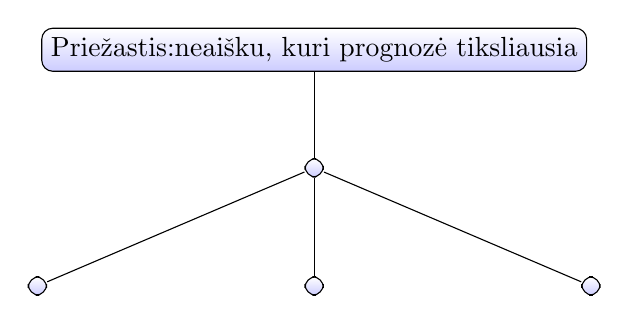
\begin{tikzpicture}[sibling distance=10em,
  every node/.style = {shape=rectangle, rounded corners,
    draw, align=center,
    top color=white, bottom color=blue!20}]]

\node(priezastis){\ent{Priežastis:}{neaišku, kuri prognozė tiksliausia}}
    child { node { \problema }
      child { node { \pasekmeI } }
      child { node { \pasekmeII } }
      child { node { \pasekmeIII } }
    };

%\node[entity] (pasekme1) [above left = of problema] {
%    \ent{Pasėkmė 1:}{žemės ūkis ruošiasi sėjai, nors artimiausias kelias dienas nelis.}
%};
%
%\node[entity] (pasekme2) [above = of problema] {
%    \ent{Pasėkmė 2:}{kelininkai ruošiasi tiesti kelio atkarpą, kurioje tuo metu lis.}
%};
%
%\node[entity] (pasekme3) [above right = of problema] {
%    \ent{Pasėkmė 3:}{išėjome į žygį, ir po pietų pradėjo lyti. O išmainėme muziejų dieną į žygį.}
%};


\end{tikzpicture}


\section{Terminai}

Tiriant ypatingus gamtos reiškinius, svarbu juos apibrėžti. Kaip pagrindą
naudosime įstatymą 111301MISAK00D1-870 \cite{lrs-stichiniai}; mums rūpimi yra
šie:

\begin{description}
    \item[Labai smarkus vėjas:] 28 m/s.
    \item[Labai smarkus lietus:] 50mm/val.
    \item[Kaitra] $>30\degree$ besitęsianti $\geq 3d$.
\end{description}

\section{Hipotezės}

\begin{itemize}
    \item To paties tiekėjo orų prognozių efektyvumas skirtingose geografinėse
        lokacijose nesikeis.
    \item Skirtingų tiekėjų orų prognozių efektyvumas bus vienodas ilguoju
        (metų) laikotarpiu.
    \item Visi tirti orų prognozių tiekėjai vienodai gerai numatys ypatingus
        gamtinius reiškinius.
\end{itemize}

\section{Tyrimo tikslo ir uždavinių nusakymas. Uždavinių medis + veiklų numatymas.}

TODO.

\section{Mokslinė literatūra, ankstesni tyrimai}

Orų prognozių tikslumas 11 metų laikotarpyje buvo analizuotas
\cite{rose2017analysis}, tačiau buvo neskirstoma tarp regionų: išvadose buvo
visi tirti kontinentai. Šiame darbe norime skirstyti prognozių tikslumą pagal
regionus, taip pat pridėti "nacionalinius" tiekėjus.

Detali literatūros apžvalga bus pridėta tolimesnėje darbo stadijoje.

\section{Metodologinė schema (tikslumo skaičiavimo metodika)}

Prognozių patikimumas bus matuojamas dviem būdais.

\subsection{Palyginamoji (bazinė) metodika}

Kad galėtume palyginti šį darbą su \cite{rose2017analysis}, "preliminariai"
analizei naudosime tuos pačius metodus:

\begin{itemize}
    \item Minimalios temperatūros paroje prognozės tikslumą.
    \item Makslimalios temperatūros paroje prognozės tikslumą.
    \item Kritulių kiekio prognozės tikslumą.
\end{itemize}

Kaip ir šaltinyje, metodika bus pritaikyta 1, 5 ir 10 dienų išankstinei
prognozei.

Šis palyginimas neatsako į pagrindinį darbo klausimą, nes neskirsto tarp
regionų. Tačiau šie duomenys yra vertingi palyginti, ar duomenys yra preliminariai
panašūs į ankstesnį darbą.

\subsection{Kartografinė metodika}

Bazinė metodika neatsako į šiuos įdomius klausimus:

\begin{itemize}
    \item Neskirsto tarp regionų: ar tarp Lietuvos regionų orų prognozės
        tikslumas skiriasi?
    \item Kuris šaltinis patikimiausiai nustato svarbius meteorologinius
        reiškinius (tarkime, $>100mm$ kritulių per 24 val.)?
    \item Kadangi patikimumą skirstome per regionus ir laiką, kaip galime tai
        informatyviai parodyti žemėlapyje?
\end{itemize}

Analizuoti ir atvaizduoti tikslumą erdvėje naudosime metodus, aprašytus
\cite{verification2015}.

Matematiniai modeliai, padėsiantys paskaičiuoti svarbių meteorologinių
reiškinių tikslumą, taip pat aprašyti \cite{verification2015}.

\section{Apibendrinimas}

Šis darbas ištirs komercinių oro tiekėjų orų prognozių patikimumą laike ir
erdvėje: minimalią, maksimalią temperatūrą, paros kritulių kiekį, ir prognozių
gebėjimą nuspėti ypatingus gamtinius reiškinius. Palyginus tyrimo rezultatus su
\cite{rose2017analysis}, taip pat tirsime ir prognozių efektyvumą per
geografinę lokaciją.

\printbibliography

\end{document}
